% !TEX encoding = UTF-8 Unicode
% !TEX root =  ../Main.tex

\chapter{Analyse und Design}\label{cha:Analyse}
Dieses Kapitel dient der Beschreibung des IST-Prozess der Antragsstellung und der Identifikation von Schwachstellen und Problemen während des Prozesses. Darauf aufbauend werden Anforderungen an das zu entwickelnde Softwareartefakt aufgestellt. Es folgt der Entwurf des Artefakts anhand der Modellierung des SOLL-Prozess, beispielhafter Darstellung der Nutzeroberfläche und dem zu Grunde liegenden Datenbankmodell.
 
\section{IST-Prozess}\label{sec:IstProzess}
Der \gls{asta} der \gls{hwr} schließt im Namen der Studierendenschaft mit einem Verkehrsanbieter einen Vertrag über den Erwerb des Semestertickets ab. Der aktuelle Vertrag wurde am 13.02.2025 mit der S-Bahn Berlin GmbH sowie der Verkehrsbund Berlin-Brandenburg GmbH geschlossen. Gemäß §1 des Vertrags sind alle ordentlich immatrikulierten Studierenden der \gls{hwr} verpflichtet, das Deutschlandsemesterticket zu beziehen. Von der Bezugspflicht ausgeschlossen sind Gasthörer:innen und Zweithörer:innen, Studierende in Abend-, Online- und Fernstudiengängen ohne Präsenzpflicht, Studierende in berufsbegleitenden und weiterbildenden Studiengängen bei denen das Studium zeitlich unterwiegt, und Studierende die nicht der Studierendenschaft angehören. \VglZitat{SemtixVertrag}{}

Zusätzlich besteht nach §4 des Vertrags für Studierende die Möglichkeit, unter foglenden Bedingungen, eine Rückerstattung des Semesterticketbeitrags beantragen: 
\begin{itemize}
  \item Urlaubssemester
  \item Auslandssemester oder Praxissemester mit einer Aufenthaltsdauer von mehr als drei zusammenhängenden Monaten außerhalb des Geltungsbereichs
  \item Doppeltimmatrikulation an zwei Hochschulen mit Semesterticketpflicht
  \item Verspätete Immatrikulation nach nach mehr als einem Monat nach Semesterbeginn
  \item Exmatrikulation im laufenden Semester
  \item Chronische Erkrankung oder Behinderung
\end{itemize}

\subsection{Prozessbeschreibung}\label{sec:Prozessbeschreibung}
Um eine Rückerstattung des Semesterticketbeitrags zu beantragen, müssen die Studierenden einen Antrag ausfüllen und diesen mitsamt Studienbescheinigung sowie erforderlicher Nachweise per E-Mail an das Sozialbüro des \gls{asta} der \gls{hwr} senden. Die Mitarbeitenden des Sozialbüros prüfen die eingereichten Dokumente zunächst auf ihre Korrektheit und Vollständigkeit. Sind Dokumente unvollständig oder fehlerhaft, werden diese bei den Studierenden per E-Mail nachgefragt. Die Dokumente vollständiger und korrekter Anträge werden mit einer Antrags-ID versehen und die Antragsdaten in einer Google-Sheets-Tabelle dokumentiert. Die Google-Sheets-Tabelle sowie alle Dokumente werden in einem privaten Google-Drive-Verzeichnis abgelegt. 

Nach Abschluss der Erstprüfung wird die E-Mail des/der Antragsstellenden mit einem Tag versehen und zur Zweitprüfung in das E-Mail-Postfach einer/eines anderen Mitarbeitenden verschoben. In der Zweitprüfung identifiziert der/die Mitarbeitende die dem Namen zugeordnet die Antrags-ID aus der Google-Sheets-Tabelle und die dazugehörigen Dokumente aus dem Google-Drive-Verzeichnis. Anschließend werden die Dokumente und die übertragenen Daten in der Google-Sheets-Tabelle ein zweites mal auf ihre Korrektheit und Vollständigkeit überprüft. Abschließend erstellt der/die Zweitprüfende mithilfe des Software-Tools Ultradox einen Bewilligungs- oder Ablehnungsbescheid. Werden Dokumente nicht nachgereicht, bleibt der Antrag unbeabeitet. 

Ablehnungen werden dem/der Studierenden unmittelbar per E-Mail zugesandt. Bei Bewilligungen erfolgt eine Weitereleitung an das Finanzteam des \gls{asta}, um den Auszahlungsprozess anzustoßen. Erst nach der Bestätigung durch das Finanzteam wird der Bewilligungsbescheid an die Studierenden versandt. Dieser Prozess ist in Abbildung~\ref{fig:istProzess} im Anhang dargestellt. 

Der aktuelle Prozess verwendet verschiedene voneinander unabhängige Softwarelösungen. Dazu gehören das E-Mail-Postfach des Sozialbüros, Google Drive als Dateisystem, Google Sheets zur tabellarischen Erfassung der Antragsdaten und Ultradox zur Erstellung der Bescheide. Bis auf Ultradox, wo die Daten aus der Google-Sheets-Tabelle nach der Auswahl der Antrags-ID automatisch aufgerufen werden, besteht zwischen den Anwendungen kein automatisierter Zusammenhang.

\subsection{Probleme und Schwachstellen}\label{sec:Probleme_und_Schwachstellen}
Bei der genauen Betrachtung des aktuellen Prozesses konnten folgende Schwachstellen identifiziert werden: 

\textbf{Hoher manueller Aufwand}\\
Wie aus der vorhergehenden Prozessbeschreibung und dem BPMN-Modell (siehe Abbildung~\ref{fig:istProzess}) deutlich wird, sind mehrere Prozesschritte manuell auszuführen:
    \begin{itemize}
    \item Das Herunterladen der eingereichten Antragsdokumente
    \item Die manuelle Benennung der Dokumente mit einer eindeutigen Antrags-ID
    \item Die Übertragung der Antragsdaten in eine Google-Sheets-Tabelle
    \item Das Hochladen der Dokumete in ein Google-Drive-Verzeichnis
    \item Taggen der E-Mail und verschieben in das Postfach des/der Zweitprüfenden
    \item Die Erstellung sowie Versand des Bewilligungs- oder Ablehnungsbescheids
    \end{itemize}
%   das Herunterladen der Antragsdokumente, die Bezeichnung des Dateinamen mit der entsprechenden Antrags-ID, die Übertragung der Antragsdaten in die Google-Sheets-Tabelle, der Upload der Antragsdokumente in das Google-Drive-Verzeichnis, das Taggen und Verschieben der E-Mail des/der Antragsstellenden in das Postfach des/der Zweitprüfenden, und die Erstellung sowie Versand des Bewilliguns- oder Ablehnungsbescheids. 
Jeder dieser Prozesschritte stellt eine potenzielle Gefahr aufgrund menschlicher Fehler dar. Beispiele dafür sind das Übersehen von Anträgen, falsche Beschriftung von Dokumente und die fehlerhafte Dateneingabe. Solche Fehler erhöhen den Arbeitsaufwand und führen zu einer Verzögerung des Auszahlungsprozesses, was wiederum Unzufriedenheit bei der Studierendenschaft auslöst. 

\textbf{Unzureichender Datenschutz nach \gls{dsgvo}}\\
Der aktuelle Antragsprozess umfasst die Verarbeitung und Speicherung personenbezogener Daten, weshalb die \gls{dsgvo} Anwendung findet (siehe Kapitel~\ref{sec:Anforderungen}). Es wurden die folgenden datenschutzrechtlichen Probleme festgestellt:  
    \begin{itemize}
    \item Es fehlt eine klare Festlegung zur Dauer der Dokumentenspeicherung (gefordert in §5 \gls{dsgvozitat}). Eine solche ist weder für die Mitarbeitenden des Sozialbüros noch die Studierendenschaft eindeutig. Informationen dazu sind weder auf der Website \VglZitat{SemtixWebsite}{},  in der Semesterticketsatzung \VglZitat{Semesterticketsatzung}{} oder der Semesterticketrichtlinie  \VglZitat{Semesterticketrichtlinie}{} zu finden.
    \item Der Schutz vor unabsichtlichem Datenverlust oder Datenveränderung (gefordert in §5 \gls{dsgvozitat}) ist nicht gewährleistet. Dokumente und Daten in dem Google-Drive-Verzeichnis sowie der Google-Sheets Tabelle können verändert und gelöscht werden, ohne die Absicherung durch Versionierungen. Ein Backup zur Wiederherstellung (gefordert in §32 Abs. 1 \gls{dsgvozitat}) gibt es nicht. 
    \item Antragsstellenden werden nicht ausreichend darüber informiert, wie ihre Daten gespeichert und verarbeitet werden. Informationen dazu sind weder auf der Website des \gls{asta} der \gls{hwr} \VglZitat{SemtixWebsite}{} noch auf dem Antrag zur Erstattung des Semestertickets zu finden (siehe Anhang~\ref{pdf:Antrag}). Die beantragende Person ist hier lediglich verpflichtet der Verarbeitung der Daten zuzustimmen.
    \item Es gibt keinen Prozess nach §33 \gls{dsgvozitat}, zur Benachrichtung der zuständigen Aufsichtsbehörde bei der Verletzung des Schutzes personenbezogener Daten. 
    \end{itemize} 
Weitere Anforderungen der \gls{dsgvo} (siehe Kapitel~\ref{sec:Anforderungen}) hingegen werden eingehalten.

\textbf{Nutzung von Google Drive}\\
In Kapitel~\ref{sec:DatenschutzGoogle} wird deutlich, dass Google LLC wenig Transparenz dazu bietet, wie und wo Daten der Nutzenden gespeichert und verarbeitet werden. Es ist nicht ersichtlich, ob die Daten innerhalb der EU gespeichert oder an Drittanbieter weitergegeben werden. Des Weiteren ist nicht deutlich, in welchem Umfang Google LLC selbst die abgespeicherten Daten zu Analysezwecken verwendet. Aus diesen Gründen ist die Verwendung von Google Drive als Dateisystem für personenbezogene Daten für einen Verwaltungsprozess ungeeignet (siehe §5 \gls{dsgvozitat}). 

% --------------------------------- ab hier Anforderungsanalyse --------------------------------------

\section{Anforderungsanalyse}\label{sec:Anforderungsanalyse}
Auf der Grundlage der zuvor beschriebenen Probleme und Schwachstellen wird im folgenden eine Anforderungsanalyse durchgeführt. Das Ziel ist es funktionale und nicht-funktionale Anforderungen einer neuen Softwarelösung zu Antragsbearbeitung zu definieren und diese als Grundlagen für Entwicklung zu verwenden. 

\textbf{Anwendungseinsatz}

Die Softwarelösung soll von Studierenden zur Antragsstellung und den Mitarbeitenden des Sozialbüros zur Antragsbearbeitung verwendet werden. Zur Nutzung der Lösung ist eine stetige Internetverbindung notwendig. Zur Nutzung der Softwarelösung soll ein Computer verwendet werden.  

\textbf{Funktionale Anforderungen}
\begin{itemize}
    \item Das System muss alle Anforderungen erfüllen, um in die aktuelle \gls{asta}-Website integriert zu werden. 
    \item Das System muss ein Formular zur Antragsstellung mit Pflichtfelder bereitstellen. Dieses Formular muss eine Upload Funktion haben, mit welcher notwendige Nachweise in Form einer PDF eingereicht werden. 
    \item Das System muss sicherstellen, dass Studierenden den Datenschutzrichtlinien zustimmen, bevor ein Antrag eingereicht werden kann. 
    \item Das System muss wenn möglich alle eingegebenen Daten auf Korrektheit prüfen. 
    \item Das System muss sicherstellen, dass der Antragsdatensatz sowie die dazugehörigen Dokumente zur eindeutigen Identifikation mit einer Antrags-ID versehen werden. 
    \item Das System muss sicherstellen, dass die Daten in einer Datenbank und die Dokumente in einem Verzeichnis abgelegt werden, auf das in einem späteren Prozessschritt zugegriffen werden kann.
    \item Das System muss sicherstellen, dass nur berechtigte Personen die Anträge einsehen können, beispielsweise durch eine rollenbasierte Rechtevergabe. 
    \item Das System muss ein Webinterface bereitstellen, über welches die Mitarbeitenden des Sozialbüros die eingegangenen Anträge bearbeiten können. 
    \item Das System muss eine Login Funktion haben, mit welcher sich die Mitarbeitenden eindeutig identifizieren können. 
    \item Das System muss sicherstellen, dass der Antragsstatus im Bearbeitungsportal automatisch und korrekt angepasst wird, sobald eine Änderung durch Mitarbeitende vorgenommen wird.
    \item Das System muss gewährleisten, dass alle Änderungen eines Antrags nachverfolgbar und nachvollziehbar sind. 
    \item Das System muss die Funktionalität haben, regelmäßig Backups der Daten erstellen zu können. 
\end{itemize}

\textbf{Nicht-funktionale Anforderungen}
\begin{itemize}
    \item Die Oberfläche soll intuitiv bedienbar sein, sodass neue Mitarbeitende schnell eingearbeitet werden können und Studierende keine Nachfragen zur Bedienung des Formulars an das Sozialbüro stellen müssen. 
    \item Das System soll alle technischen und organisatorischen Maßnahmen der \gls{dsgvo} berücksichtigen, insbesondere §32 \gls{dsgvozitat}.
\end{itemize}

\textbf{Abgrenzungskriterien}

Die folgenden Kriterien sind zum aktuellen Zeitpunkt nicht Bestandteil des geplanten Softwareartefakts. Es handelt sich hierbei teilweise um Maßnahmen, die zum realen Einsatz der Software durch das Sozialbüro notwendig sind und deren Realisierung in einer späteren Entwicklungsphase geplant ist. 
\begin{itemize} 
    \item Die Möglichkeit, nach der Zweitprüfung eines Antrags, den Bewilligungs- oder Ablehnungsbescheid  direkt über das Bearbeitungsportal generieren zu lassen (beispielsweise durch die Anbindung an Ultradox). 
    \item Der automatische Versand der Bewilligungs- oder Ablehnungsbescheide an das Finanzteam sowie den/die Studierende:n. 
    \item Eine Funktion zur automatischen Nachforderung von Dokumenten, wenn Anträge unvollständig sind. 
    \item Eine Anbindung an die Datenbank der \gls{hwr} um eine eindeutige Identifikation der Studierenden zu gewährleisten und mögliche Angriffe zu vermeiden. 
    \item Die Möglichkeit in dem Formular digital zu unterschreiben, um die Rechtmäßigkeit des Antrags zu gewährleisten. 
\end{itemize}


% --------------------------------- ab hier Soll-Prozess und UI --------------------------------------

\section{Systementwurf}\label{sec:Systementwurf}
Der folgende Abschnitt dient der Beschreibung SOLL-Prozess, der sich durch die Integration des zu entwickelnden Softwareartefakts ergibt. 
Die bisherige Antragsstellung per E-Mail wird vollständig durch ein webbasiertes Onlineformular auf der \gls{asta}-Website abgelöst. Dadurch entfallen manuellen Arbeitsschritte, wie das Öffnen von E-Mails, das Zuweisen einer Antrags-ID und das Eintragen der Antragsdaten in die Google-Sheets Tabelle. 

Eingehende Anträge werden den Mitarbeitenden des Sozialbüros im Bearbeitungsportal mit dem Status \glqq{}Neu\grqq{} angezeigt. Über die Benutzeroberfläche können die Daten sowie hochgeladene Dokumente eingesehen werden. Die Mitarbeitenden entscheiden per Auswahlfunktion, ob ein Antrag bewilligt oder abgelehnt wird. Entsprechend ändert sich der Status zu \glqq{}Erstprüfung - Bewilligt\grqq{} oder \glqq{}Erstprüfung - Abgelehnt\grqq{}. 

Im nächsten Prozessschritt erfolgt die Zweitprüfung. Stimmen die Entscheidungen von Erstprüfenden und ZWeitprüfenden überein, wird der Status des Antrags automatisch auf \glqq{}Zweitprüfung - Bewilligt\grqq{} bzw. \glqq{}Zweitprüfung - Abgelehnt\grqq{} gestzt. Stimmen die Entscheidungen nicht überein, erhält der Antrag den Status \glqq{}Erneute Prüfung notwendig\grqq{}. 

Geplant, aber nicht Teil der aktuellen Implementierung ist die Möglichkeit, nach der Zweitprüfung automatisiert einen Bescheid generieren zu lassen und diesen direkt an den/die Studierenden und das Finanzteam weiterzuleiten. 

Die Kommunikation mit Studierenden erfolgt weiterhin per E-Mail. Wenn Unterlagen fehlen oder diese unvollständig sind, müssen diese nachgefordert werden. Die Mitarbeitenden des Sozialbüros haben dafür die Möglichkeiten einen Antrag per Knopfdruck auf den Status \glqq{}Dokumente nachgefordert\grqq{} zu setzen, auch diese Funktion soll in der Zukunft automatisiert werden, ist jedoch nicht Teil der aktuellen Lösung. Anträge, die bis spätestens 30 Tage vor Semesterende nicht vollständig eingereicht wurde, werden auf den Status \glqq{}Archiviert\grqq{} gesetzt. Der gesamte Prozess von Antragseinreichung durch das Online-Formular auf der \gls{asta} Website über die Bearbeitung des Antrags bis hin zum Versandt des Bescheids ist in Abbildung~\ref{fig:sollProzess} im Anhang dargestellt.

\subsection{Antragsformular}\label{sec:Antragsformular_entwurf}
Das Antragsformular, über welches die Studierenden ihren Antrag einreichen können umfasst eine Reihe von Pflichtfeldern: 
\begin{multicols}{2}
\begin{itemize}[noitemsep, topsep=4pt]
    \item Vorname
    \item Nachname
    \item Matrikelnummer
    \item Hochschul-E-Mail-Adresse
    \item Straße
    \item Hausnummer
    \item Postleitzahl 
    \item Ort 
    \item zu beantragendes Semester
    \item Erstattungsgrund
    \item IBAN 
    \item BIC 
    \item Bankname
    \item Zustimmung zu den AGBs 
    \item Zustimmung zur Verarbeitung der personenbezogenen Daten
\end{itemize}
\end{multicols}

Abbildung~\ref{fig:antragsformular} zeigt eine mögliche Visualisierung des Antragsformulars. Eine größere Darstellung der Abbildung ist im Anhang zu finden. 

\begin{figure}[htbp]
  \centering
  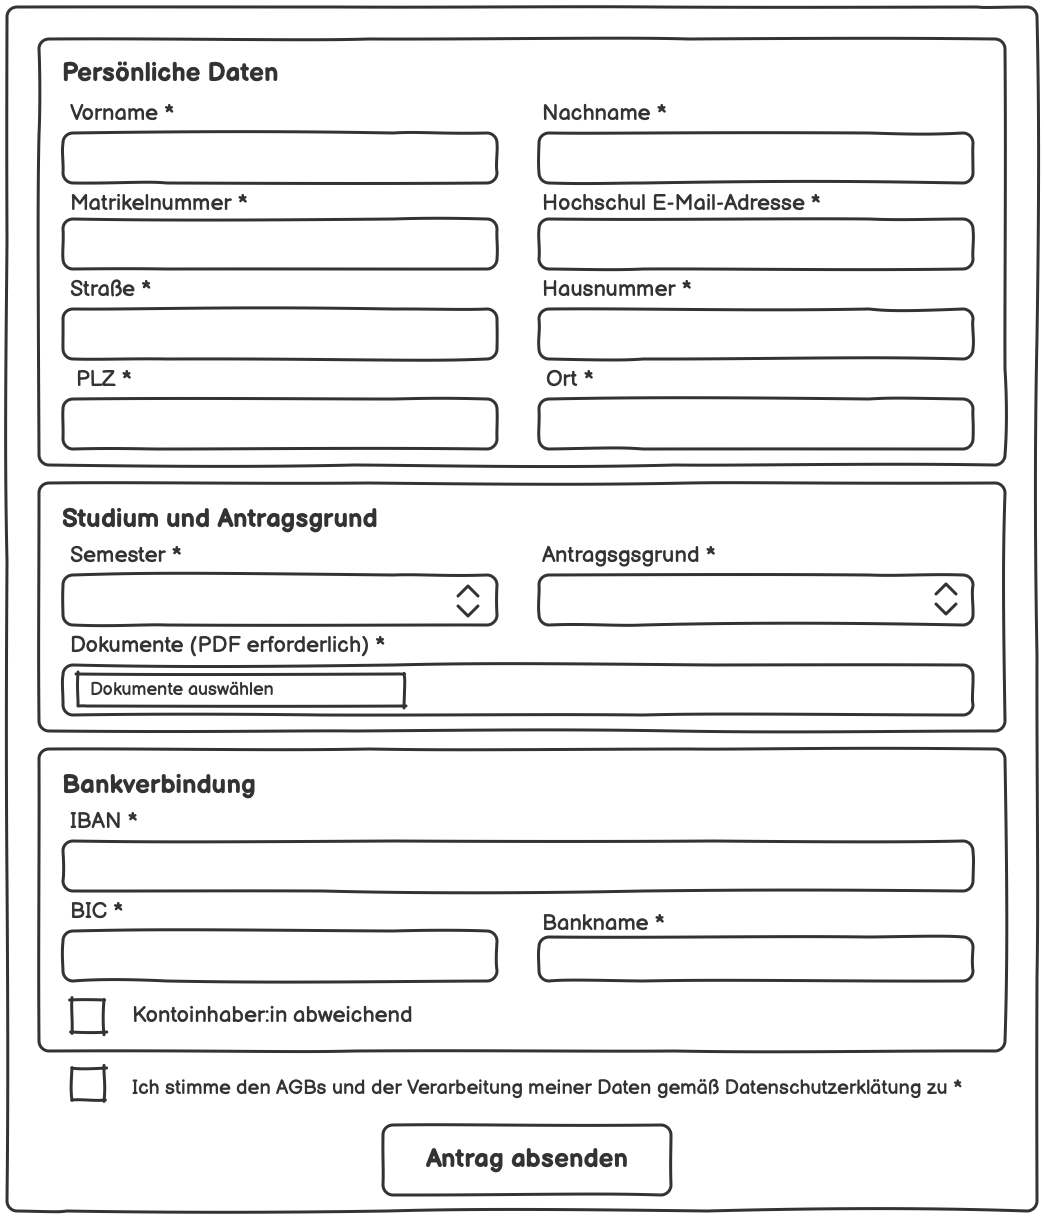
\includegraphics[width=0.7\textwidth]{Bilder/Antragsformular.png}
  \caption{User Interface des Antragsformulars}\label{fig:antragsformular}
\end{figure}

\subsection{Bearbeitungsportal}\label{sec:Bearbeitungsportal}
Das Bearbeitungsportal für die Mirarbeitenden des Sozialbüros bildet den Kern der Lösung. Wenn der/die Nutzende die Webapplikation aufrufen, wird er/sie auf der ersten Seite aufgefordert, sich einzuloggen. Nach dem Login wird der/die Mitarbeitende zur Antragsübersicht weitergeleitet. Hier werden alle Anträge angezeigt, sortiert nach Antrags-ID. Es gibt die Möglichkeit die Anträge nach ihrem Status zu filtern, um den Mitarbeitende die Arbeit übersichtlicher zu machen. Abbildung~\ref{fig:Antragsübersicht} zeigt eine mögliche Darstellung dieser Seite. Eine größere Darstellung der Abbildung ist im Anhang zu finden. 

\begin{figure}[htbp]
  \centering
  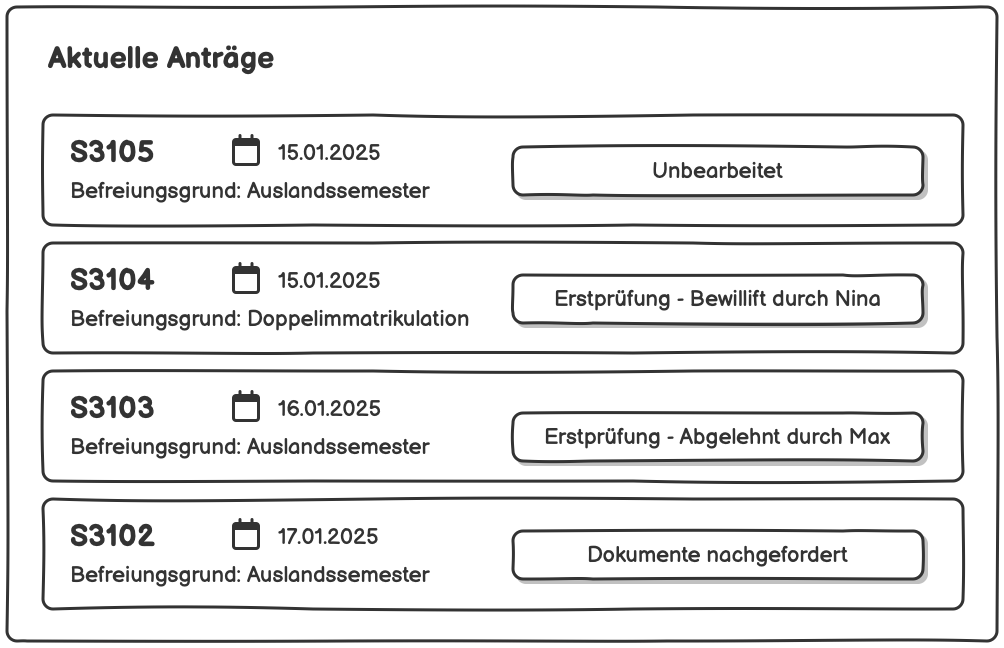
\includegraphics[width=0.7\textwidth]{Bilder/Aktuelle_Anträge.png}
  \caption{User Interface des Bearbeitungsortals auf der Seite \glqq{}Antragsübersicht\grqq{}}\label{fig:Antragsübersicht}
\end{figure}


Zur Bearbeitung eines Antrags muss die Detailansicht geöffnet werden (siehe Abbildung~\ref{fig:detailAnträge}, eine größere Darstellung der Abbildung ist im Anhang zu finden). Auf dieser werden alle von dem/der Studierenden sowie die hochgeladenen Dokumente angezeigt. Hier haben die Mitarbeitenden die Möglichkeit, den Antrag zu bearbeiten und den Status zu verändern, wie in Kapitel~\ref{sec:Systementwurf} beschrieben. 

\begin{figure}[!htb]
  \centering
  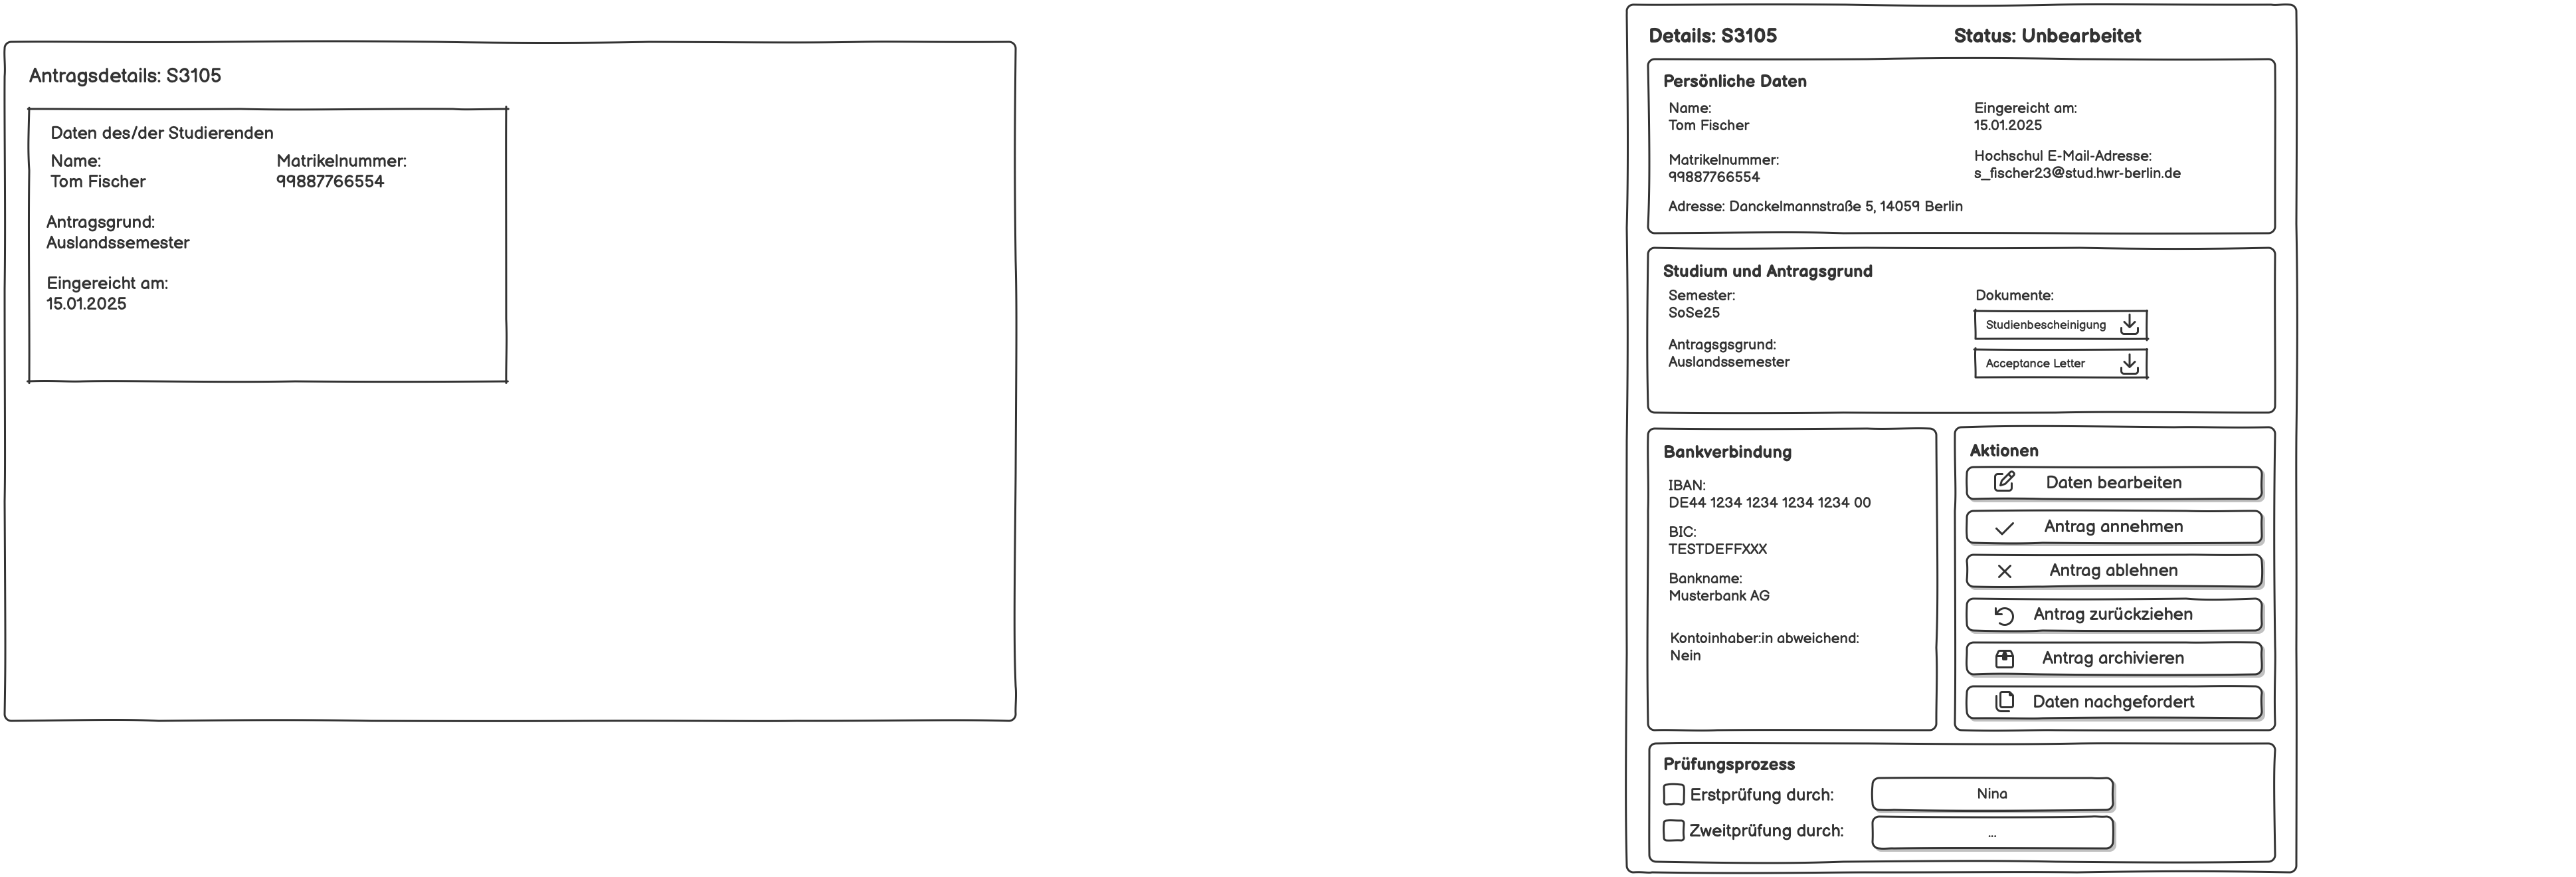
\includegraphics[width=0.7\textwidth]{Bilder/Detail_Antrag.png}
  \caption{Detailansicht eines Antrags}\label{fig:detailAnträge}
\end{figure}

% --------------------------------- ab hier Datenmodell --------------------------------------

\subsection{Datenmodell}\label{sec:Datenmodell}
Zum Aufbau einer Datenbankstruktur ist es sinnvoll, ein Datenbankschema zu entwickeln. Ein solches konzeptionelles Schema ist das \gls{erm}. Als Entität ist ein Objekt zu verstehen, welches verschidene Charakteristika haben kann. Mehrere Entitäten mit den gleichen Eigenschaften werden als Entitätsmenge zusammengefasst. Bei einer Entitätsmenge ist es deshalb notwendig, ein Attribut zu bestimmen, welches die Entitäten voneinander unterscheidet. Das kann Beispielsweise eine ID sein. Diese Entitätsmengen sind durch Beziehungen verknüpft, welche wiederum selbst Merkmale haben können. Ein solches \gls{erm} kann dann auf eine Datenbank abgebildet werden. \VglZitat{SQL}{29 ff.} Ein \gls{erm} zum Antragsprozess ist in Abbildung~\ref{fig:erm} dargestellt. Die Abbildung ist vergrößert im Anhang dargestellt. Es gibt folgende Entitätsmengen: 
\begin{description}
  \item[Student:in:] Das ist die Person, welche den Antrag stellt. Neben einer eindeutigen ID werden auch die personenbezogenen Daten als Attribute gespeichert. Eine Person kann pro Semester nur einen Antrag stellen. 
  \item[Antrag:] Der Antrag ist das Kernstück. Es werden das Semester, Antragsgrund und Antragsdatum sowie die Bankdaten gespeichert. Ein Antrag beinhaltet mehrere Dokumente und er kann verschiedene Bearbeitungszustände während des Prozesses annehmen. 
  \item[Mitarbeiter:in:] Hierbei handelt es sich um die Personen, die einen Antrag prüfen, den Status ändern und den dazugehörigen Bewilligungs- oder Ablehnungsbescheid erstellen. 
  \item[Bearbeitungshistorie:] Die Bearbeitungshistorie dokumentiert die Änderungen eines Antrags während des Prüfprozesses. Jede Änderung des Status wird mit dem Änderungsdatum sowie dem/der Mitarbeiter:in festgehalten, um den Prozess nachvollziehbar zu machen. 
  \item[Bescheid:] Ein Antrag kann bewilligt oder abgelehnt werden (muss er aber nicht). Geschieht das, wird ein Bescheid von einem/einer Mitarbeitenden erstellt. Jeder Antrag kann nur einen Bescheid haben.   
\end{description}

\begin{figure}[htbp]
  \centering
  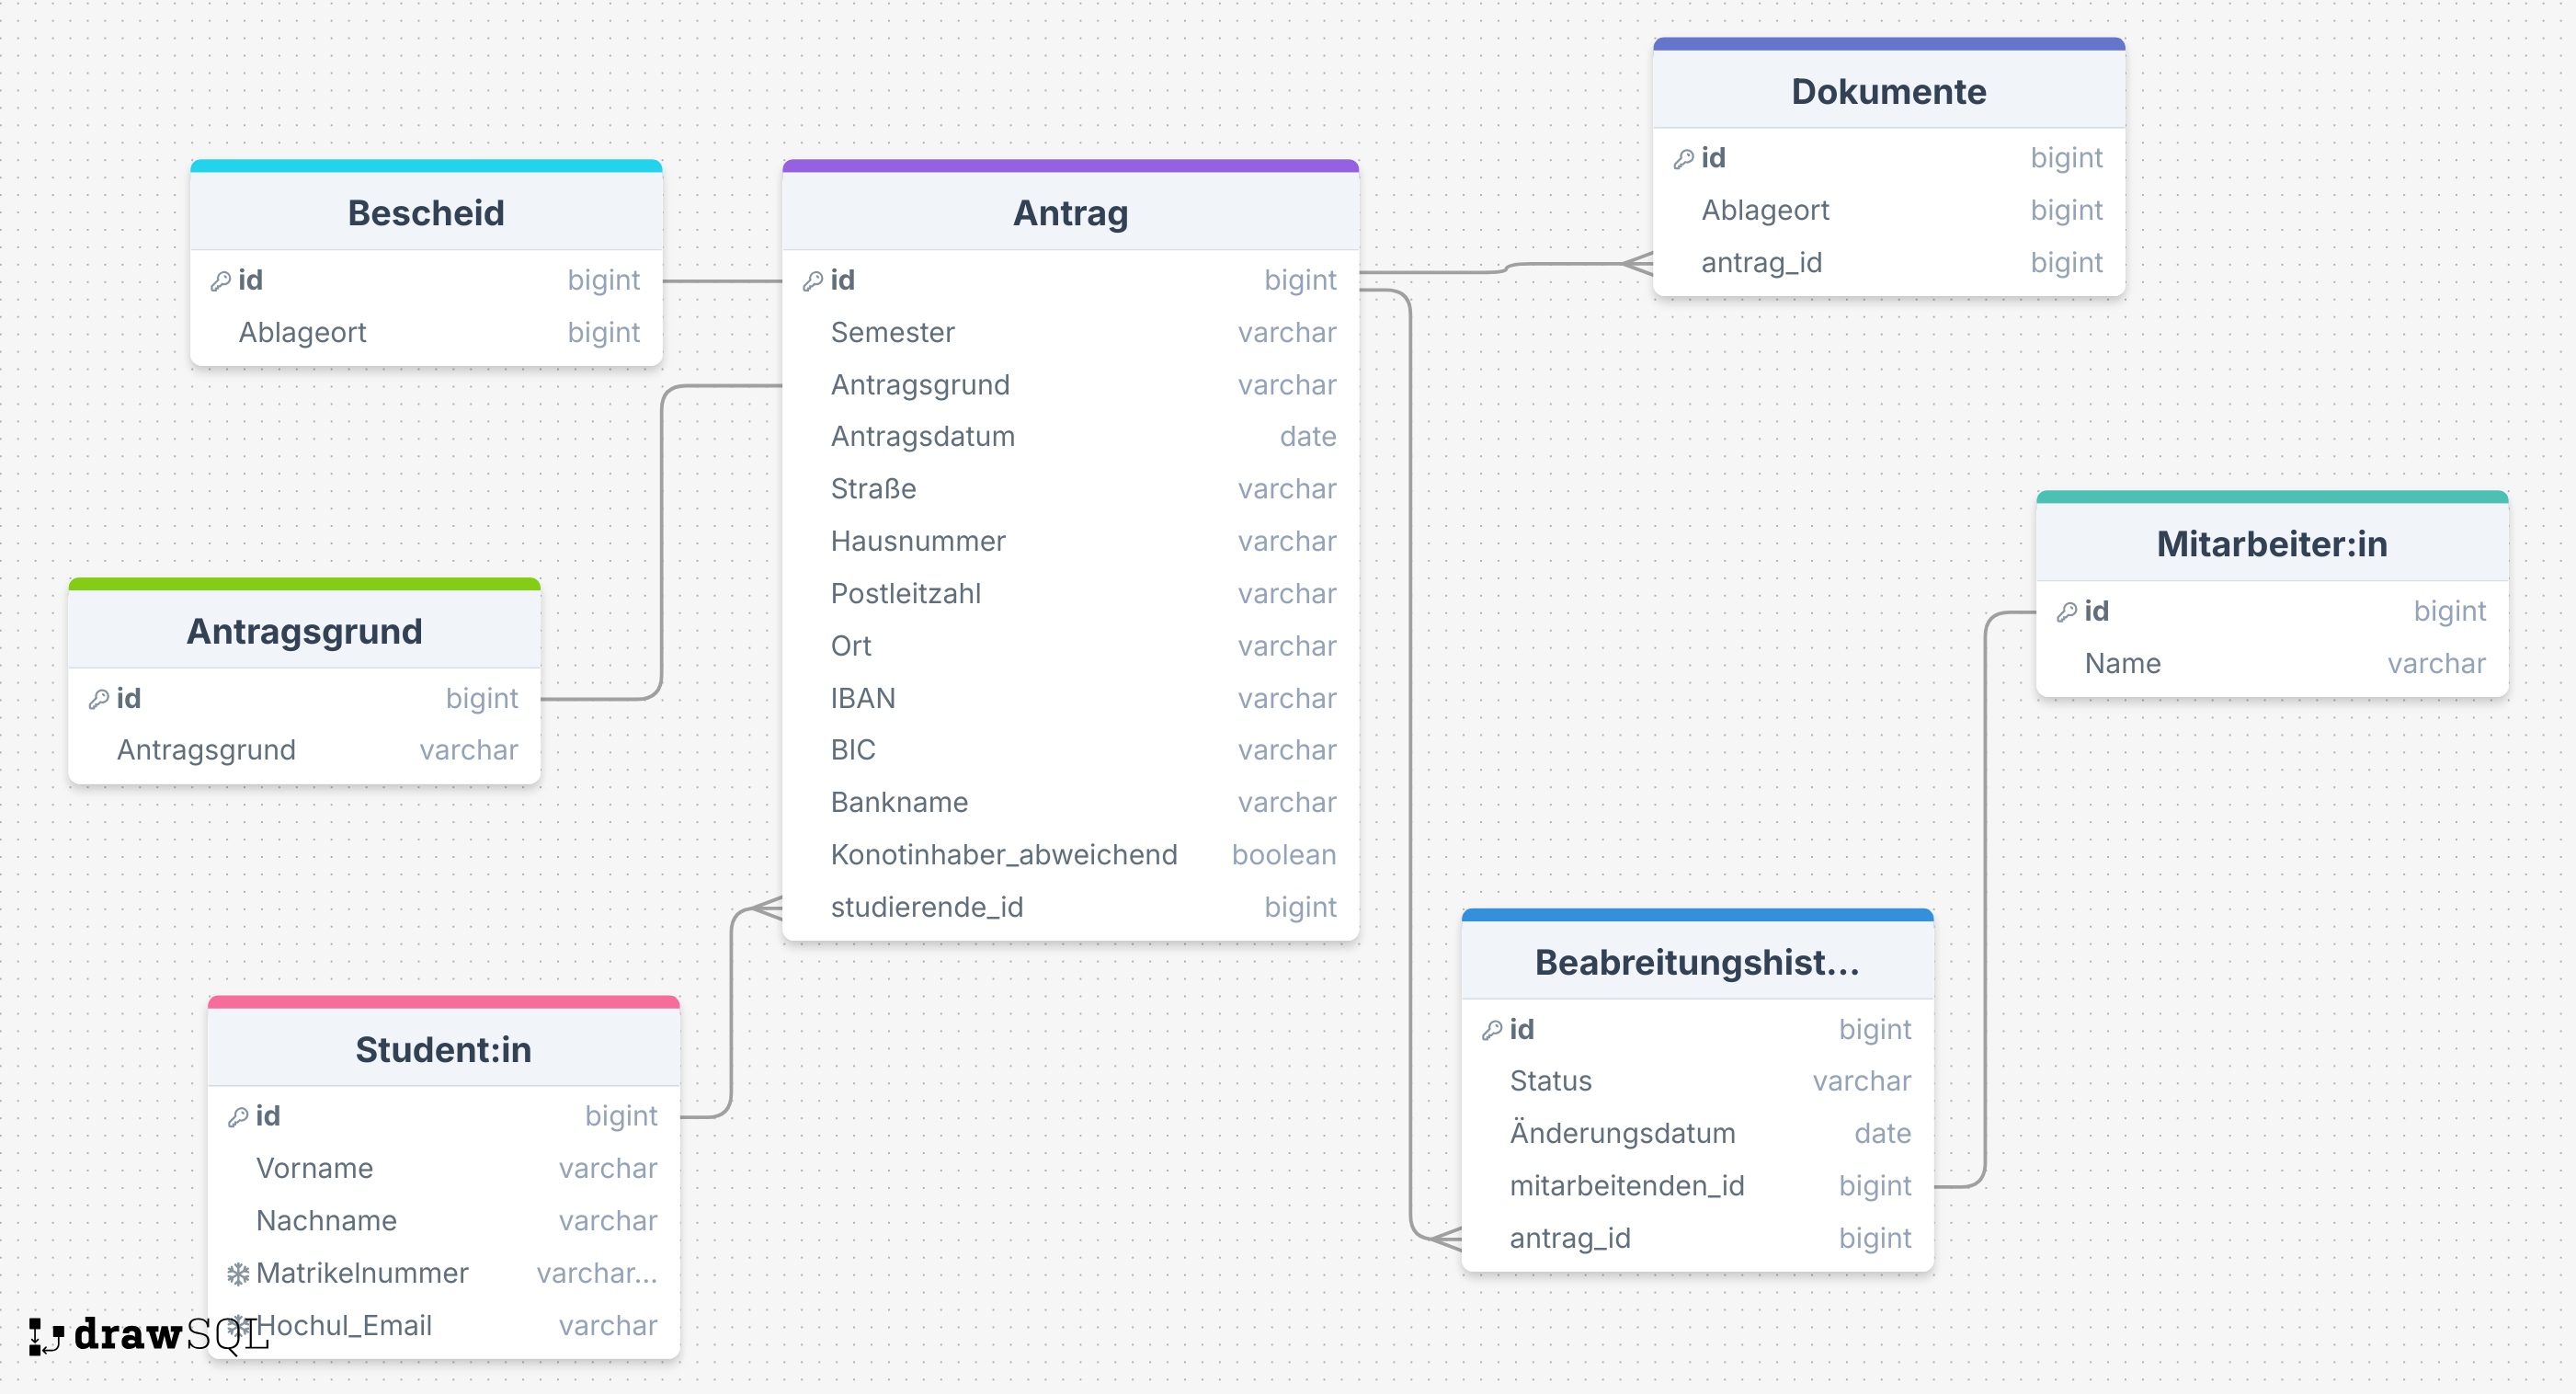
\includegraphics[width=1\textwidth]{Bilder/ERM.png}
  \caption{\gls{erm} des Antragsprozesses}\label{fig:erm}
\end{figure}

Das in Abbildung~\ref{fig:erm} dargestellte \gls{erm} bildet die Grundlage für die technische Umsetzung der Datenbank. Um die dargestellten Entitten und Beziehungen in einer relationalen Datenbank zu speichern, müssen sie in eine relationales Modell überführt werden. Dieses Modell stellt Daten in Form von Tabellen da, wobei jede Tabelle eine Menge von Datensätzen mit festen Spalten (Attributen) enthält. Bei der Überführung des \gls{erm} müssen bestimmte Abbildungsregeln beachtet werden \VglZitat{SQL}{49 ff.}:
\begin{enumerate}
  \item Jede Entitätsmenge muss einen Primärschlüssel, also ein eindeutiges Attribut aufweisen.
  \item Jede Beziehungsmenge kann ebenfalls eine eigene Tabelle haben. Diese Tabelle muss keinen Primärschlüssel enthalten, er kann auch durch Fremdschlüssel der Entitätsmengen gebildet werden.
  \item Komplex-komplexe Beziehungsmengen (also m zu n Beziehungen) benötigen eine eigenständige Tabelle.
  \item Einfach-komplexe Beziehungsmengen benötigen keine eigenständige Tabelle. Es reicht aus, dass der Primärschlüssel als Fremdschlüssel in der Ausgangstabelle verwendet wird.
  \item Auch einfach-einfache Beziehungsmengen benötigen keine eigenständige Tabelle. Hier wird ebenfalls der Primärschlüssel als Fremdschlüssel in der Ausgangstabelle referenziert.
\end{enumerate}

Nach der Anwendung dieser Abbildungsregeln auf das erstellte \gls{erm} entstand ein Datenbankmodell, wonach die Tabellen der Datenbank beschrieben in Kapite~\ref{sec:Datenbank} erstellt uwrden. Dieses Datenbankmodell befindet sich als Abbilung~\ref{fig:datenbankmodell} im Anhang. 



% Das Relationsmodell beschreibt Daten und ihre Beziehungen zueinander in Form von Tabellen. Daraus hervorgehend entstanden relationale Datenbanken. Relation mein hier nicht, wie umgangssprachlich  verstanden, eine \glqq{}Beziehung\grqq{}, sondern eine Teilmenge aller möglichen Kombinationen der Werte der Attribute, wobei eine Relation als $R$ und die Mengen der Werte der Attribute mit $D_n$ bezeichnet werden.
% Mathematisch lässt sich das so ausdrücken:
% \[
% R \subseteq D_1 \times D_2 \times \dots \times D_n
% \]
% Eine Relation ist auch eine Menge sogenannter Tupel. Ein Tupel $r$ ist eine Menge konkreter Datenwerte, also Ausprägungen der Attribute $D_i$. Die Menge aller Tupel einer Relation lässt sich wie folgt darstellen:
% \[
% R = \{ r_1, r_2, \dots, r_m \}
% \]
% Augrund des mathematischen Mengenbegriffs, darf ein Tupel nicht mehrfach vorkommen. Deshalb ist es sinnvll eine eindeutiges Attribut wie eine ID als Primärschlüssel hinzuzufügen. \VglZitat{SQL}{41 f.}